\section{Proposed Method}
\label{sec:methods}
In this section, we introduce the multi-modal caption generation pipeline and the proposed feature learning framework.
%
\textcolor{red}{Fig.}~\ref{fig:Dataset} illustrates the details of caption generation, including attribute definitions and examples.
%
\textcolor{red}{Fig.}~\ref{fig:Overall} presents the key modules of our proposed IDEA: the Inverted Multi-modal Feature Extractor (IMFE) and the Cooperative Deformable Aggregation (CDA).
%
Details are described as follows.
%
\begin{figure*}[t]
    \centering
      \resizebox{1.0\textwidth}{!}
      {
    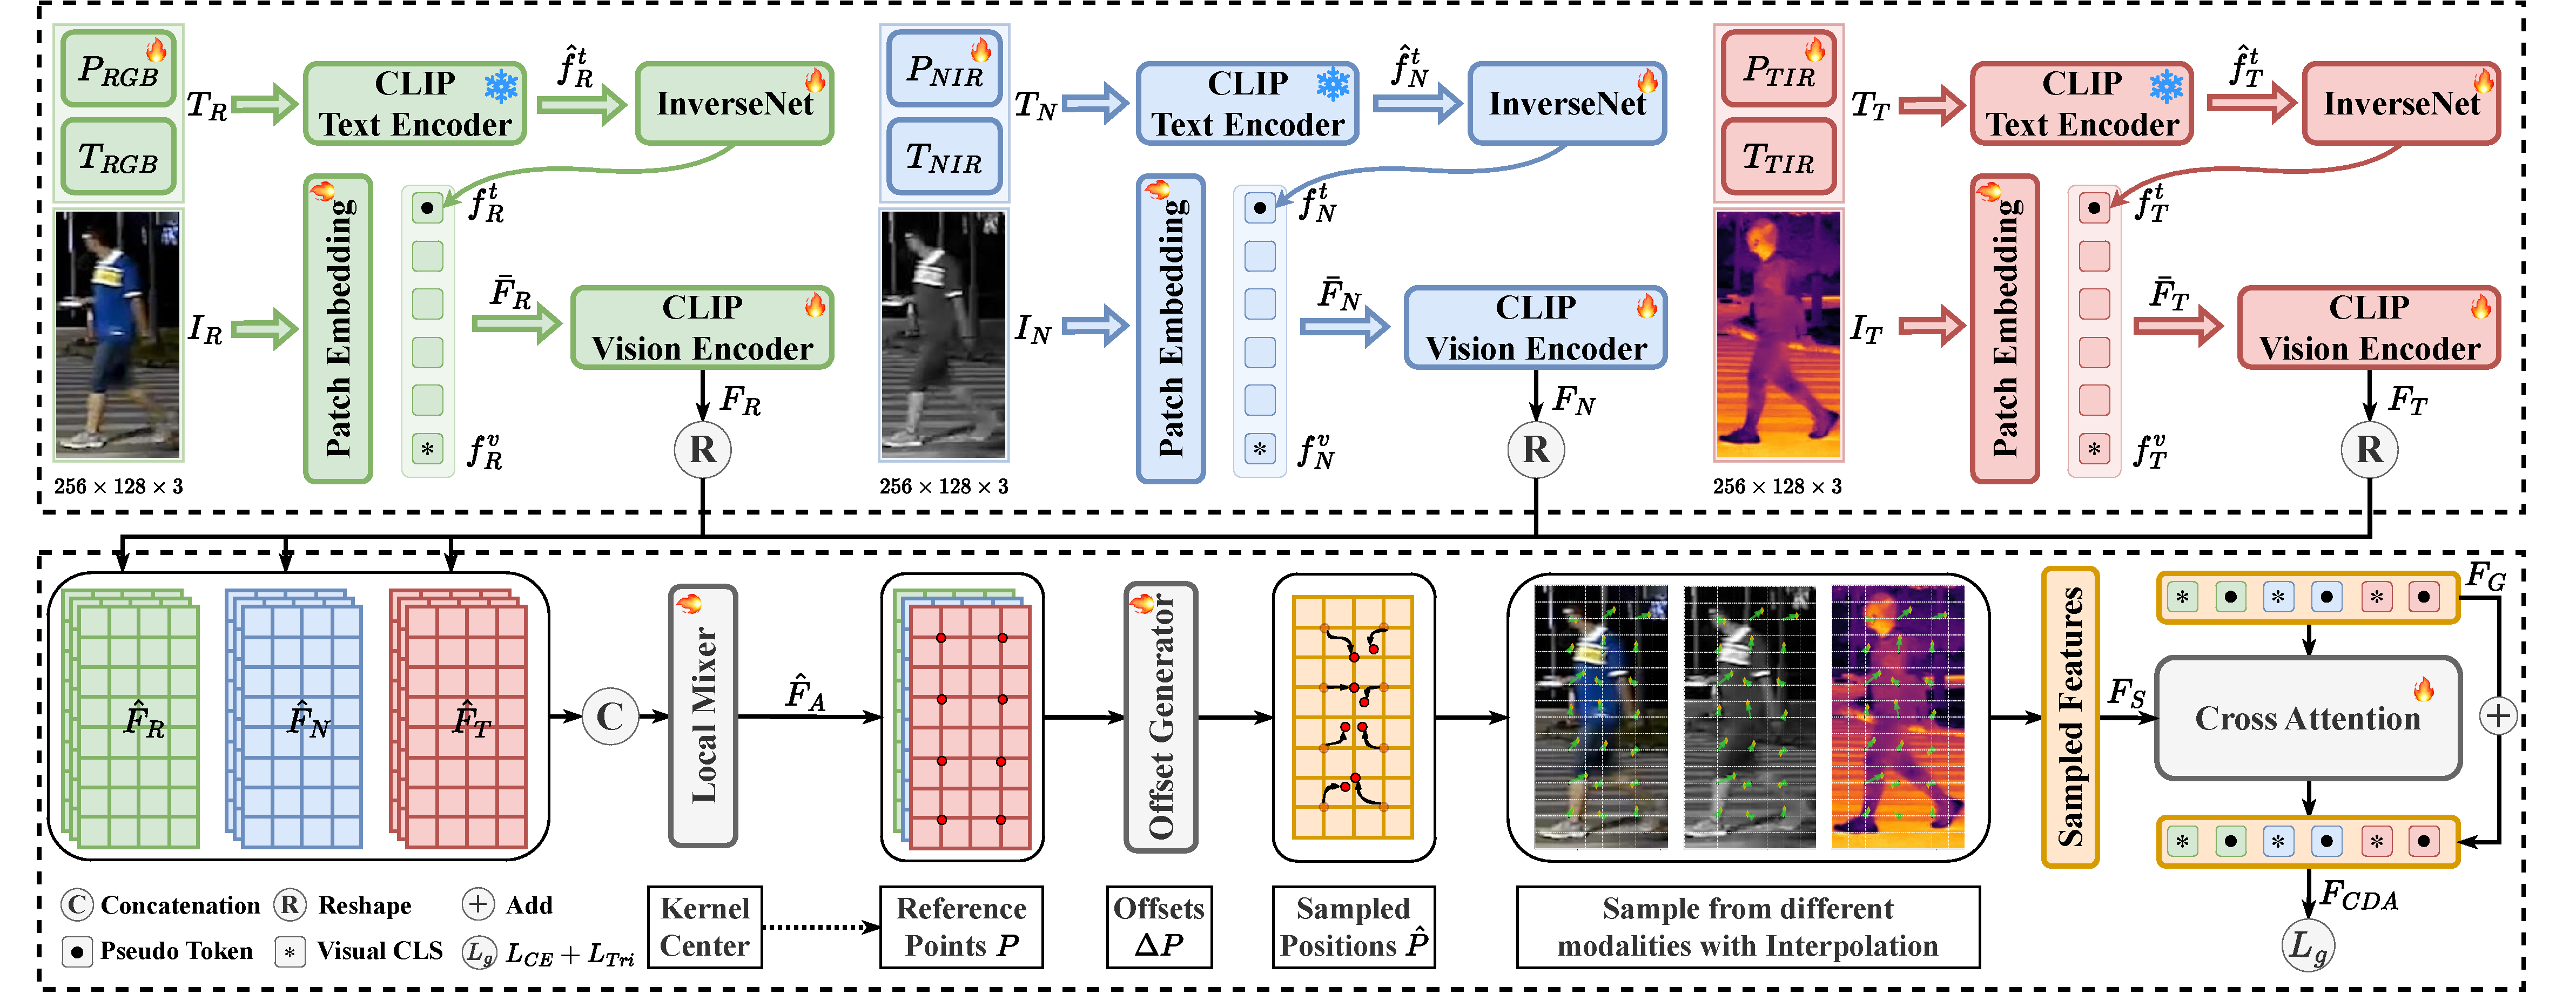
\includegraphics[width=30\linewidth]{sec/img/Overall.pdf}
    }
    \vspace{-4mm}
     \caption{Illustration of the proposed IDEA framework.
     %
     The upper part depicts the Inverted Multi-modal Feature Extractor (IMFE).
     %
     It employs modal prefixes and an InverseNet to incorporate semantic text guidance for feature discriminability.
     %
     The lower part highlights the Cooperative Deformable Aggregation (CDA), which adaptively integrates discriminative local information with global features.
     %
     With the integration of IMFE and CDA, IDEA effectively extracts discriminative multi-modal features for object ReID.}
    \label{fig:Overall}
    \vspace{-2mm}
  \end{figure*}
  %~~~~~~~~~~~~~~~~~~~~~~~~~~~~~~~~
\subsection{Multi-modal Caption Generation}
To bridge the gap in multi-modal text annotation, we propose the Multi-modal Caption Generation pipeline.
%
To be specific, our pipeline consists of two steps.
%
The first step generates informative descriptions, while the second step reuses the MLLMs to extract the predefined key attributes.
%
\\
\textbf{Caption Generation.}
%
Taking our person annotation as an example, we define 8 attribute categories in \textcolor{red}{Fig.} \ref{fig:Dataset} (a), including gender, belongings and so on.
%
These attributes are mapped into the template shown in the top part of \textcolor{red}{Fig.} \ref{fig:Dataset} (a).
%
To tailor the description to each modality, we add specific prefixes: \textit{“Write a comprehensive description of the person's overall appearance based on the [RGB/NIR/TIR] image, ...”}.
%
Besides, we incorporate commands to prevent the hallucination of the MLLMs~\cite{tan2024harnessing}, forming a complete prompt.
%
This prompt, along with the corresponding image, is fed into the MLLMs to generate the textual description.
%
\\
\textbf{Attribute Extraction.}
After obtaining an initial description, we feed it back into the MLLMs to extract predefined attributes.
%
After that, we populate these attributes into the same template we used for caption generation, forming a structured and concise description.
%
As shown in \textcolor{red}{Fig.}~\ref{fig:Dataset} (b), the descriptions for each modality can align well with the corresponding images.
%
For instance, the \textit{“white t-shirt”} and \textit{“purse”} in the RGB image are accurately captured.
%
For the vehicle dataset, we follow similar pipelines.
%
As illustrated in \textcolor{red}{Fig.}~\ref{fig:Dataset} (c), the text of the RGB image successfully captures the license plate number \textit{“KQQ819”}.
%
Meanwhile, the car logo is more prominent in the TIR image, with \textit{“Hyundai”} being identified.
%
This approach allows us to establish a unified pipeline for multi-modal text annotation, ensuring structural descriptions across different modalities.
\subsection{IDEA Framework}
\subsubsection{Inverted Multi-modal Feature Extractor}
To leverage the semantic guidance from texts, we propose the Inverted Multi-modal Feature Extractor (IMFE).
%
Unlike previous methods~\cite{wang2024top,zhang2024magic} that focus on fusing multi-modal images, we incorporate multi-modal texts into the fusion.
%
However, as indicated by the \textcolor{blue}{blue keywords} in \textcolor{red}{Fig.}~\ref{fig:Dataset} (b) and (c), conflicts can arise due to the nature of multi-modal images.
%
Directly aggregating contradictory information can lead to model confusion.
%
Thus, IMFE employs Modal Prefixes and an InverseNet to address these issues.\\
\textbf{Modal Prefixes.}
To enhance the model’s awareness of different modal texts and mitigate the impact of conflicting information, we propose a simple method called Modal Prefixes.
%
Taking the text input for the RGB branch as an example, as shown in the top left corner of \textcolor{red}{Fig.}~\ref{fig:Overall}, $T_{RGB}$ represents the text annotation of the RGB image, while $P_{RGB}$ is the modal prefix for RGB modality.
%
$P_{RGB}$ consists of two parts: a fixed text describing the characteristics of the RGB image and learnable tokens for fine-tuning.
%
Specifically, $P_{RGB}$ is structured as: \textit{“An image of a XXXX person in the visible spectrum, capturing natural colors and fine details: ”}, where \textit{“XXXX”} is replaced by an equal number of learnable tokens~\cite{li2023clip}.
%
Here, we denote the number of learnable tokens as $N_{P}$.
%
Then, we concatenate $P_{RGB}$ and $T_{RGB}$ to form the text input $T_{R}$ for the RGB branch:
\begin{equation}
    T_{R} = [P_{RGB}, T_{RGB}].
\end{equation}
Other modalities follow the same structure to guide the model in distinguishing between different modal texts.
%
With this simple yet effective method, the model can better understand the characteristics of each modality and reduce conflicts during multi-modal fusion.
\\
\textbf{InverseNet.}
To fully leverage the semantic information from texts, we propose the InverseNet.
%
Previous methods~\cite{baldrati2023zero,han2024clip} often reverse global image information into pseudo-text tokens and use texts as the primary modality for downstream tasks.
%
However, due to the limitations of MLLMs and the complexity of multi-modal image annotations, the generated texts may contain some errors and conflicts.
%
To address this, we take a different direction, reversing global text information into pseudo-image tokens.
%
In this reversal, we also incorporate rich information from the learnable tokens in Modal Prefixes.
%
This approach enables the interaction between semantic information and image details, resulting in a discriminative feature representation.
%

Specifically, as shown in the upper part of \textcolor{red}{Fig.}~\ref{fig:Overall}, the text $T_{m}$ is first fed into the CLIP's text encoder $\mathcal{T}$ for extracting the semantic feature $\hat{f}^{t}_{m} \in \mathbb{R}^{C}$ as follows:
%
\begin{equation}
    \hat{f}^{t}_{m} = \mathcal{T}(T_{m}).
\end{equation}
Here, $m \in \{R, N, T\}$ represents the RGB, NIR and TIR modalities, respectively.
%
$C$ denotes the embedding dimension.
%
If learnable tokens exist in the modal prefixes, $\hat{f}^{t}_{m}$ will be updated by the average of learnable tokens.
%
Then, we feed $\hat{f}^{t}_{m}$ into the InverseNet $\mathcal{I}$ to generate the pseudo token $f^{t}_{m} \in \mathbb{R}^{C'}$ with the following equation:
\begin{equation}
    f^{t}_{m} = \mathcal{I}(\hat{f}^{t}_{m}).
\end{equation}
Here, $C'$ is the dimension of the pseudo token \textbf{while $\mathcal{I}$ is essentially a simple layer of MLP}.
%
Meanwhile, for the image input $I_{m}$, we first patchify it into $N_l$ patches.
%
Then, we concatenate the pseudo token \( f^{t}_{m} \), the patch tokens and a learnable token \( f^{v}_{m} \) to form the image feature \( \bar{F}_{m} \in \mathbb{R}^{(N_l + 2)\times C'} \).
%
Finally, we feed \( \bar{F}_{m} \) into the CLIP's vision encoder \( \mathcal{V} \) to obtain the integrated feature \( F_{m} \in \mathbb{R}^{(N_l + 2) \times C} \) as follows:
\begin{equation}
    F_{m} = \mathcal{V}(\bar{F}_{m}).
\end{equation}
By incorporating the InverseNet, we can effectively leverage the semantic information from texts and enhance the discriminability of the feature representation.

\subsubsection{Cooperative Deformable Aggregation}
To effectively extract discriminative local information and adaptively aggregate complementary multi-modal features, we propose Cooperative Deformable Aggregation (CDA).
%
% Existing methods~\cite{wang2022interact,wang2024top} often involve interactions using all patch tokens across modalities, leading to two challenges: high computational cost and vulnerability to noise in local patches, which can undermine feature robustness during multi-modal fusion.
%
CDA addresses the noise interference by adaptively generating sampling positions of key local regions.
%
This module enables interactions between global features and discriminative local features, ensuring efficient feature aggregation.

Technically, as illustrated in the lower part of \textcolor{red}{Fig.}~\ref{fig:Overall}, we first extract patch tokens from the integrated feature \( F_{m} \).
%
These patches are then reshaped to form \( \hat{F}_{m} \in \mathbb{R}^{H \times W \times C} \), where \( H \) and \( W \) represent the height and width of the local feature map, respectively.
%
Next, we concatenate these features along the channel dimension and pass them into the Local Mixer \( \mathcal{M} \) for interaction.
%
Specifically, \( \mathcal{M} \) comprises point-wise convolution \( \mathcal{P} \), the GELU activation function~\cite{hendrycks2016gaussian} \( \delta \) and depth-wise convolution \( \mathcal{D} \).
%
This process yields the aggregated local features \( \hat{F}_{A} \in \mathbb{R}^{H_{S} \times W_{S} \times C} \):
%
\begin{equation}
    \hat{F}_{A} = \mathcal{M}([\hat{F}_{R}, \hat{F}_{N}, \hat{F}_{T}]),
\end{equation}
\begin{equation}
  \mathcal{M}(\mathcal{X}) = \delta(\mathcal{D}(\delta(\mathcal{P}(\mathcal{X})))),
\end{equation}
%
where \([\cdot]\) means concatenation.
%
\( H_{S} \) and \( W_{S} \) represent the number of sampled regions in the height and width dimensions, respectively.
%
Since the convolution \( \mathcal{D} \) aggregates local information in the receptive field of the kernel, we define the center of each convolution operation as the reference points \( P \in \mathbb{R}^{H_{S} \times W_{S} \times 2} \).
%
Based on these reference points, the aggregated local information is then used to determine the direction in which the model should shift within the local region.
%
Thus, we send \( \hat{F}_{A} \) into the Offset Generator \( \mathcal{G} \) to predict the offsets \( \Delta{P} \in \mathbb{R}^{H_{S} \times W_{S} \times 2} \) as follows:
%
\begin{equation}
    \Delta{P} = \mathcal{G}(\hat{F}_{A}) * k,
\end{equation}
%
where \( k \) scales the offset magnitude~\cite{xia2022vision} and \( \mathcal{G} \) denotes a linear layer.
%
Finally, we apply the offsets \( \Delta{P} \) to the reference points \( P \) to get the sampling locations \( \hat{P} \in \mathbb{R}^{H_{S} \times W_{S} \times 2} \), which are \textbf{shared across modalities}~\cite{zhang2024magic}:
\begin{equation}
    \hat{P} = P + \Delta{P}.
\end{equation}
Next, we sample the local features \( \hat{F}_{m} \) at the positions \( \hat{P} \) using the bilinear interpolation to obtain the discriminative local features.
%
The features are concatenated to form the sampled feature \( F_{S} \in \mathbb{R}^{3N_{S} \times C} \), where \( N_{S} = H_{S} \times W_{S} \) represents the number of sampled regions.
%
At this stage, we utilize the cooperative information from multiple modalities to generate deformable local discriminative features.
%
As illustrated by the sampling points visualization in \textcolor{red}{Fig.}~\ref{fig:Overall}, the adaptive offsets effectively concentrate on critical semantic regions of the human body, enhancing the discrimination.
%

To promote the interaction between global features and discriminative local features, we incorporate cross attention~\cite{dosovitskiy2020image}.
%
Specifically, we extract the visual class token and pseudo token from the integrated feature \( F_{m} \) to construct the global feature \( F_{G} \in \mathbb{R}^{6 \times C} \).
% Pseudo token only 1 in each modality
Then, the global feature \( F_{G} \) is used as the query, while the sampled local feature \( F_{S} \) serves as the key and value to facilitate interaction:
\begin{equation}
    F_{CDA} = F_{G} + \mathcal{CA}(F_{G}, F_{S}),
\end{equation}
%
where \( F_{CDA} \in \mathbb{R}^{6 \times C} \) represents the final feature while \( \mathcal{CA} \) denotes the cross attention block.
%
By incorporating the CDA, we can effectively extract discriminative local information and adaptively aggregate complementary multi-modal features, enhancing the model’s discriminability.
%
\subsection{Objective Function}
As shown in \textcolor{red}{Fig.}~\ref{fig:Overall}, we optimize IDEA through losses applied to multiple features.
% where \( F_{G} \) is used to optimize IMFE and \( F_{CDA} \) focuses on optimizing CDA.
%
To maintain consistency with prior works~\cite{wang2024top,zhang2024magic}, we separately extract image and text features from \( F_{G} \) and \( F_{CDA} \), resulting in \( F^{v}_{G}, F^{t}_{G} \) and \( F^{v}_{CDA}, F^{t}_{CDA} \in \mathbb{R}^{3C} \).
%
For each feature, we apply label smoothing cross-entropy loss~\cite{szegedy2016rethinking} and triplet loss~\cite{hermans2017defense}:
\begin{equation}
    \mathcal{L}_{g}(\mathcal{F}) = \mathcal{L}_{CE}(\mathcal{F}) + \mathcal{L}_{Tri}(\mathcal{F}),
\end{equation}
where \( \mathcal{F} \) denotes the input feature.
%
Here, \( \mathcal{L}_{CE} \) is the label smoothing cross-entropy loss while \( \mathcal{L}_{Tri} \) means the triplet loss.
%
The overall objective function is then formulated as:
\begin{equation}
    \mathcal{L} = \mathcal{L}_{g}(F^{v}_{G}) + \mathcal{L}_{g}(F^{v}_{CDA}) + \mathcal{L}_{g}(F^{t}_{G}) + \mathcal{L}_{g}(F^{t}_{CDA}).
\end{equation}
\vspace{-8mm} 